%%=====================================================================
%% RESULTADOS E DISCUSSÃO (TCC, cap. 4). Números conferidos com
%% ../TCC_documento/Textuais/Resultados e Conclusao/01_Discussao.tex
%% Uma figura ou tabela por slide; a fala fica no roteiro.md.
%%=====================================================================
\secaoudesc{Resultados e discussão}

%% --- parâmetros do motor -------------------------------------------
\begin{frame}{Parâmetros elétricos do motor}
  \centering
  \begin{fundobranco}
  \begin{tabular}{lccc}
    \toprule
    \textbf{Grandeza} & \textbf{Método} & \textbf{Linha} & \textbf{Fase (estrela)} \\
    \midrule
    Resistência & Kelvin, 12 pontos & \SI{17,37 \pm 0,02}{\milli\ohm} & \SI{8,69 \pm 0,01}{\milli\ohm} \\
    Indutância  & Ressonância $LC$, 3 capacitores & \SI{13,90 \pm 0,14}{\micro\henry} & \SI{6,95 \pm 0,07}{\micro\henry} \\
    Indutância  & Ajuste harmônico, 16 registros & -- & \SI{11,3}{\micro\henry} \\
    \bottomrule
  \end{tabular}
  \end{fundobranco}
  \fonte
\end{frame}

%% --- sensor de corrente --------------------------------------------
\begin{frame}{Sensor de corrente: montagem do ensaio}
  \centering
  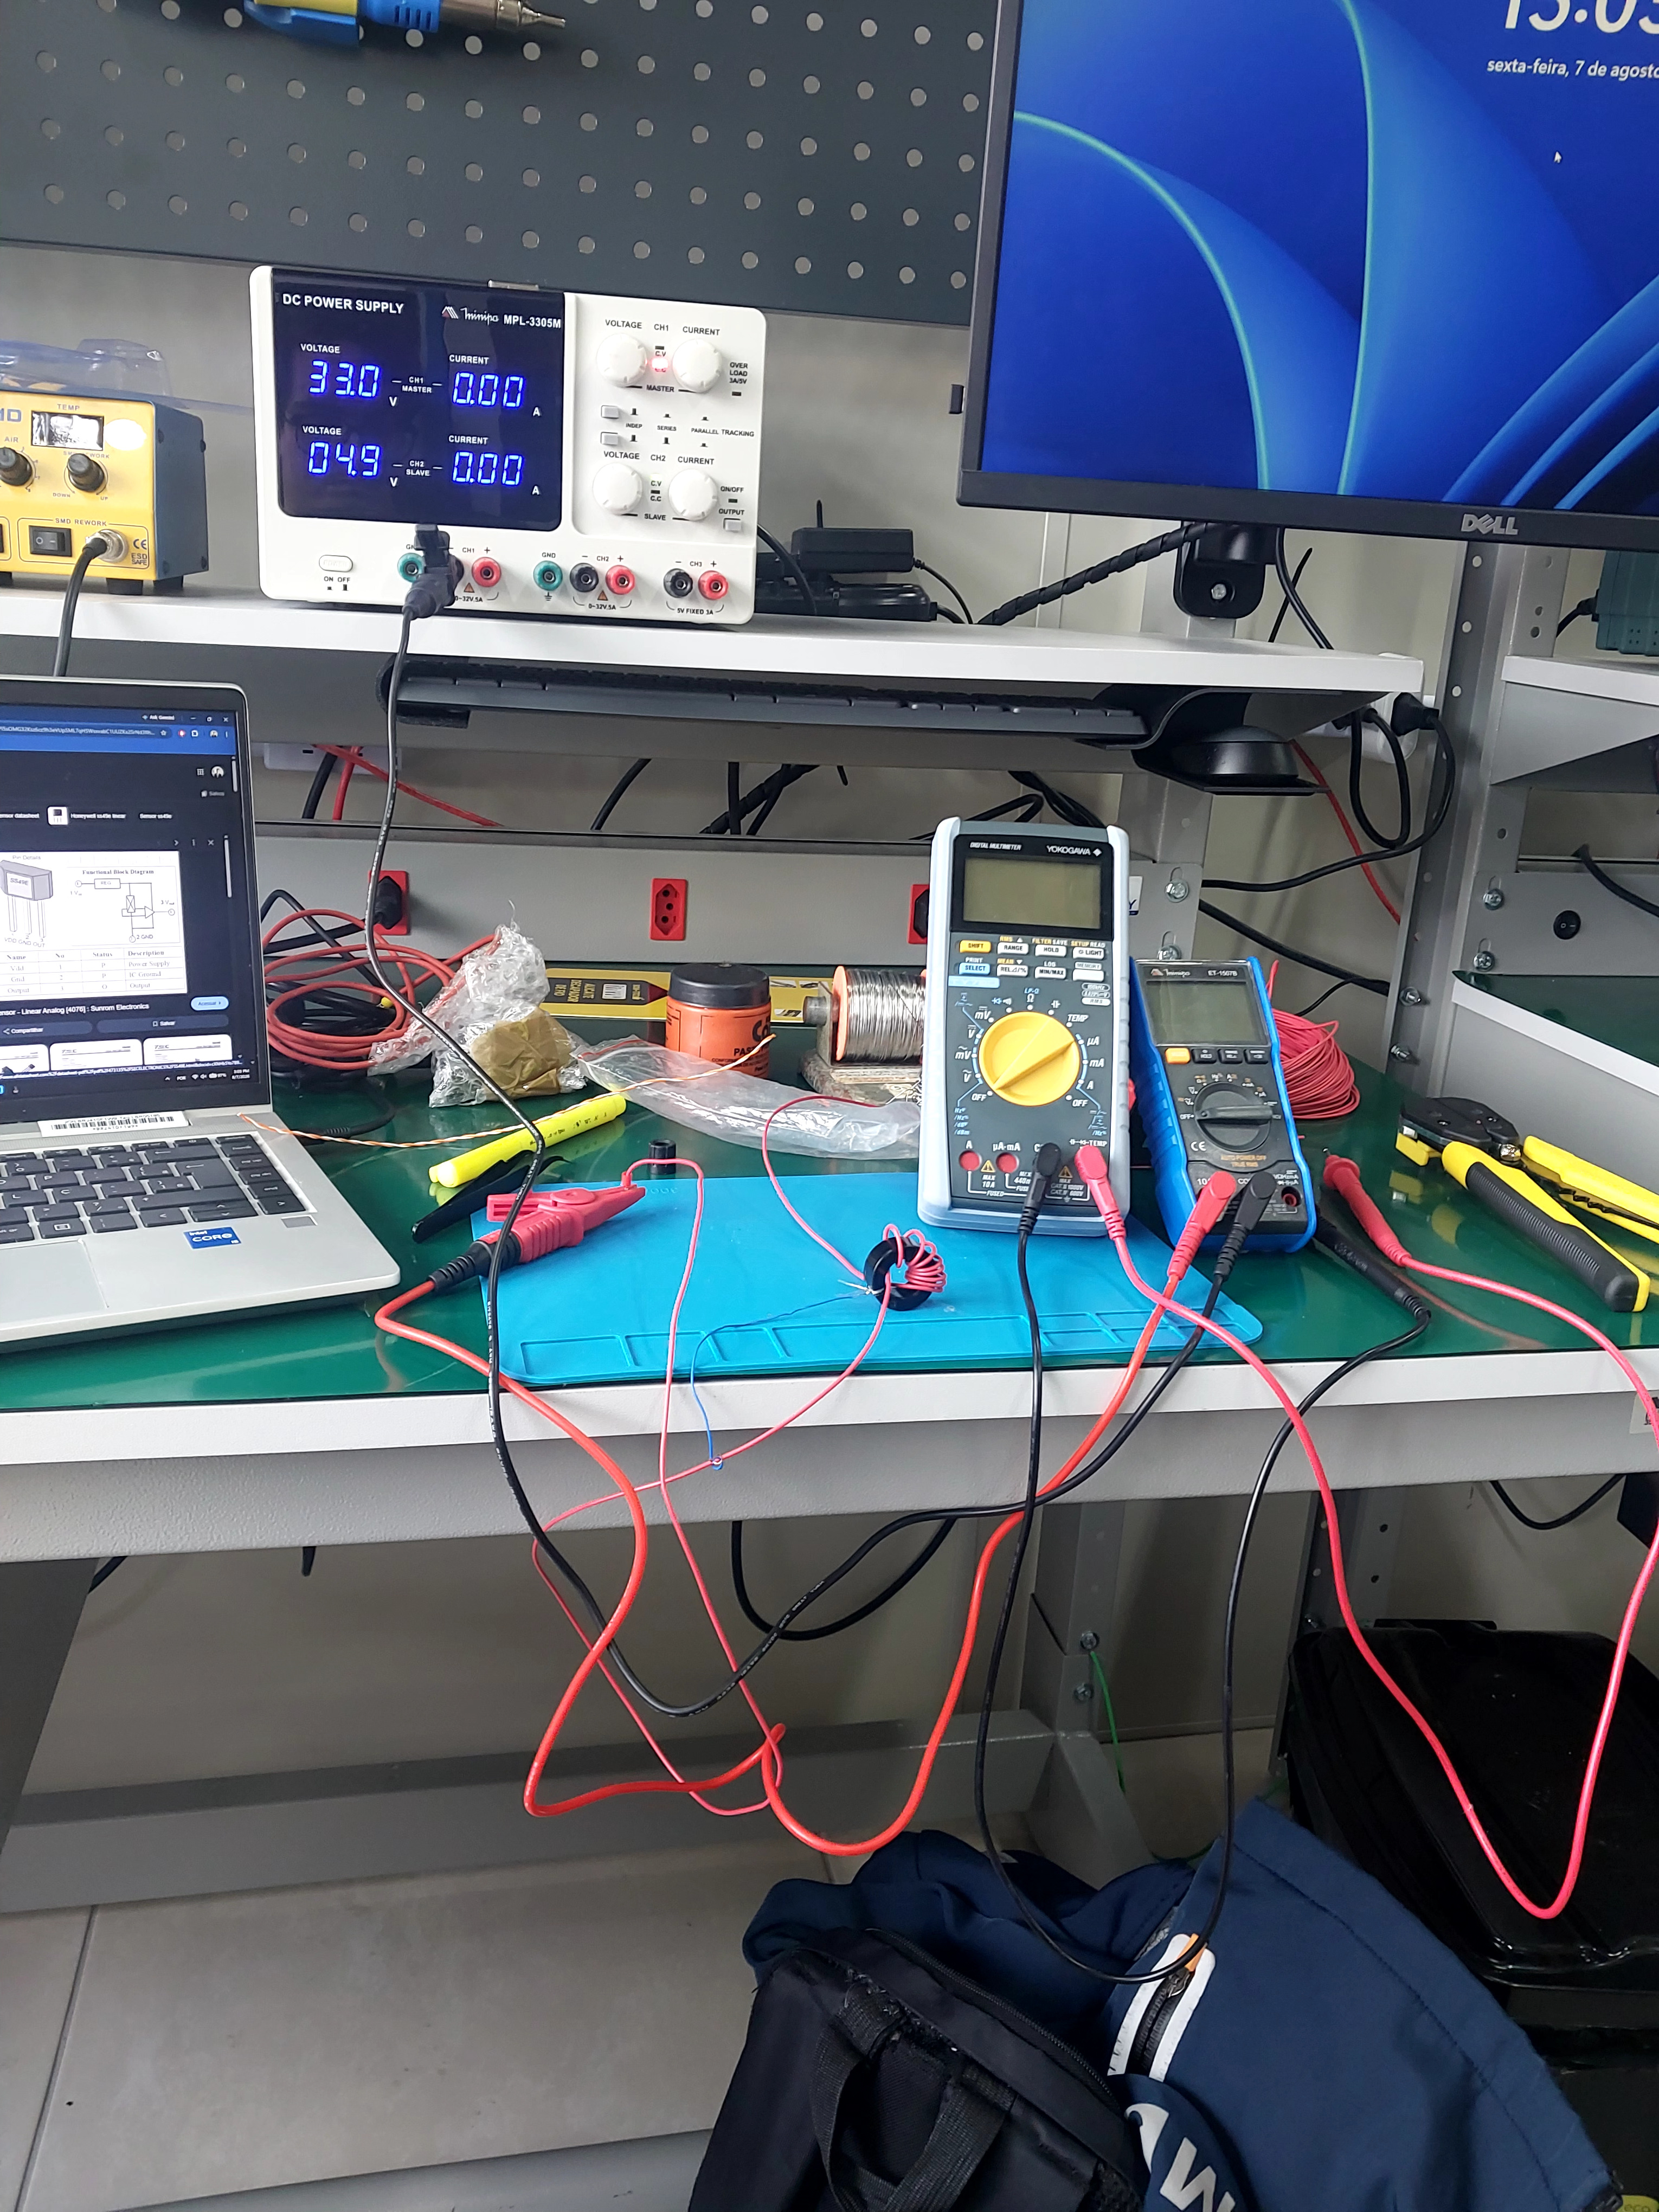
\includegraphics[width=\linewidth,height=0.75\textheight,keepaspectratio]{Resultados/ensaio_sensor_corrente.jpg}
  \fonte
\end{frame}

\begin{frame}{Sensor de corrente: tensão de saída $\times$ corrente}
  \centering
  \tikzfig{1}{0.75}{sensor_vout_i}
  \fonte
\end{frame}

\begin{frame}{Sensor de corrente: curva $\Delta V \times B$}
  \centering
  \tikzfig{1}{0.75}{sensor_dv_b}
  \fonte[Autor (2026); Honeywell International Inc.\ (2016)]
\end{frame}

\begin{frame}{Sensor de corrente: parâmetros por configuração}
  \centering
  \begin{fundobranco}
  \begin{tabular}{cccccc}
    \toprule
    $N$ & $B$ varrido [G] & $S$ [\si{\milli\volt\per\ampere}] &
    $S_H$ [\si{\milli\volt\per\gauss}] & Desvio do típico & $R^2$ \\
    \midrule
    1 & 0 -- 78  & \num{18,75 \pm 0,16}  & \num{1,209} & \SI{-13,6}{\percent} & \num{0,99939} \\
    4 & 0 -- 330 & \num{90,87 \pm 0,09}  & \num{1,465} & \SI{+4,7}{\percent}  & \num{0,99999} \\
    8 & 0 -- 516 & \num{165,42 \pm 0,20} & \num{1,334} & \SI{-4,7}{\percent}  & \num{0,99999} \\
    \midrule
    \multicolumn{3}{l}{Média das três configurações} & \num{1,336} & \SI{-4,6}{\percent} & -- \\
    \multicolumn{3}{l}{Típico de catálogo} & \num{1,400} & -- & -- \\
    \bottomrule
  \end{tabular}
  \end{fundobranco}
  \fonte[Autor (2026); Honeywell International Inc.\ (2016)]
\end{frame}

%% --- simulação ------------------------------------------------------
%% --- simulação do observador (TCC 4.3) ------------------------------
\begin{frame}{Simulação: desempenho do PLL (hélice APC 17x10E)}
  \centering
  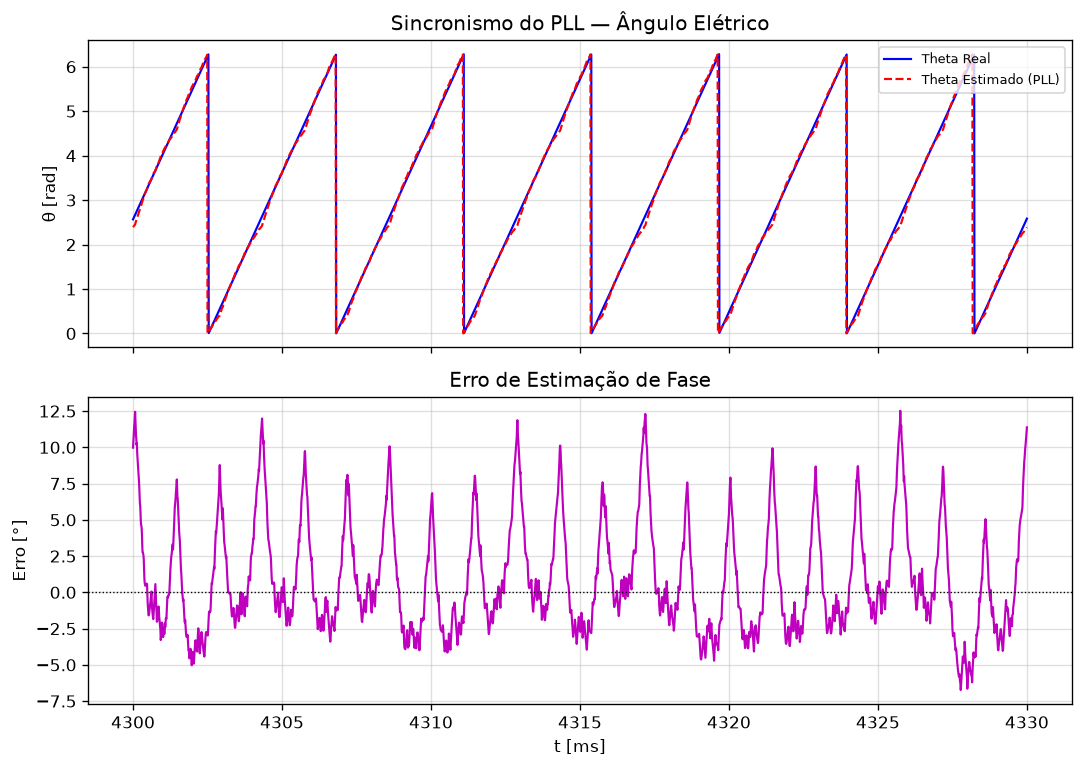
\includegraphics[width=\linewidth,height=0.75\textheight,keepaspectratio]{Desenvolvimento/PLL_angulos.png}
  \fonte
\end{frame}

\begin{frame}{Ajuste automático: convergência da otimização (APC 17x10E)}
  \centering
  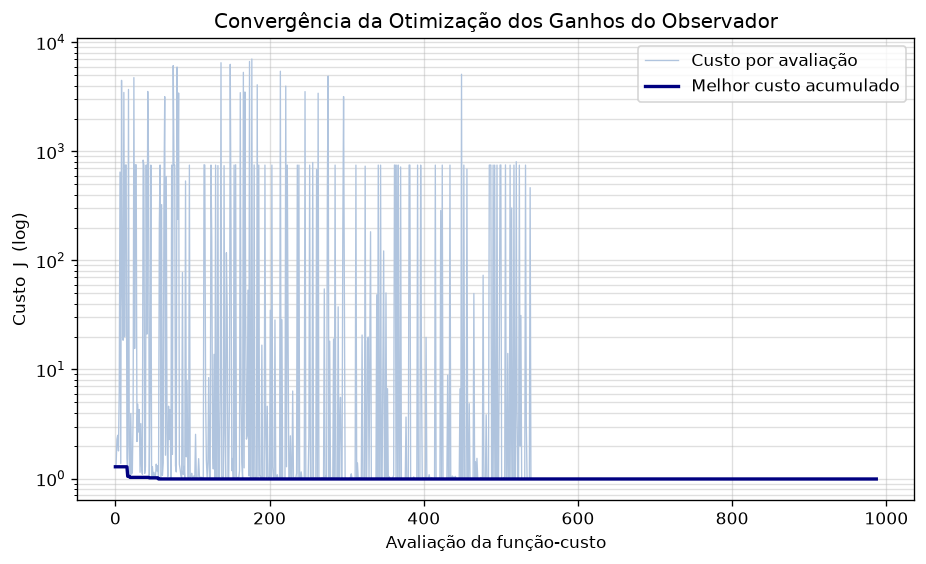
\includegraphics[width=\linewidth,height=0.75\textheight,keepaspectratio]{Desenvolvimento/Otim_convergencia.png}
  \fonte
\end{frame}

\begin{frame}{Ajuste automático: ganhos obtidos por hélice}
  \centering
  \begin{fundobranco}[0.85]
  \begin{tabular}{lcccc}
    \toprule
    \textbf{Hélice} & $\Gamma_{s1}$ & $\Gamma_{s2}$ & $\Gamma_t$ &
    \textbf{Custo final / inicial} \\
    \midrule
    APC 15x6E  & \num{20,73} & \num{-10,00} & \num{0,0037} & \num{1,013} / \num{1,300} \\
    APC 17x10E & \num{26,55} & \num{-10,00} & \num{0,095}  & \num{0,992} / \num{1,280} \\
    \bottomrule
  \end{tabular}
  \end{fundobranco}
  \fonte
\end{frame}

\begin{frame}{Ajuste automático: sensibilidade da função-custo a cada ganho}
  \begin{columns}[t]
    \begin{column}{0.33\textwidth}
      \centering
      {\small (a) $\Gamma_{s1}$}\\[0.2em]
      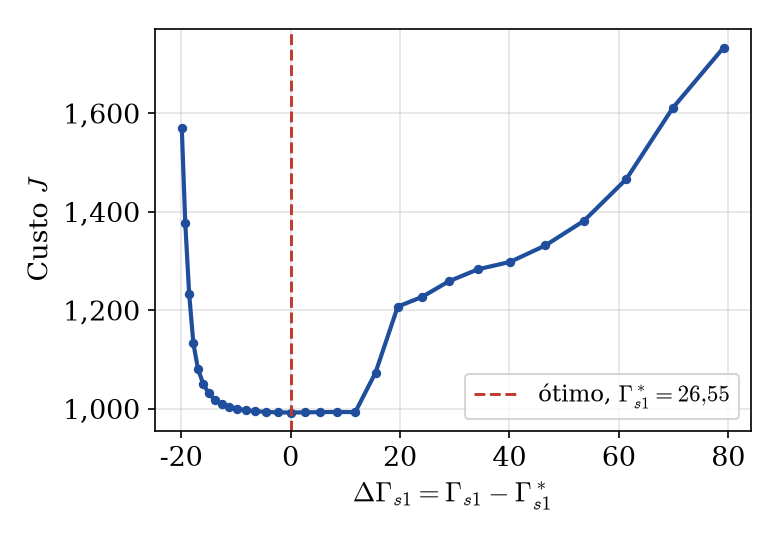
\includegraphics[width=\linewidth]{Desenvolvimento/Otim_sensibilidade_s1.png}
    \end{column}
    \begin{column}{0.33\textwidth}
      \centering
      {\small (b) $\Gamma_{s2}$}\\[0.2em]
      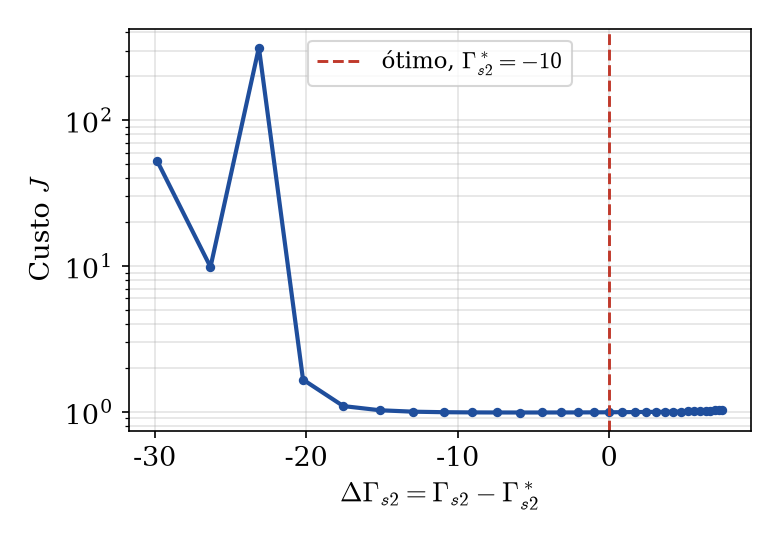
\includegraphics[width=\linewidth]{Desenvolvimento/Otim_sensibilidade_s2.png}
    \end{column}
    \begin{column}{0.33\textwidth}
      \centering
      {\small (c) $\Gamma_{t}$}\\[0.2em]
      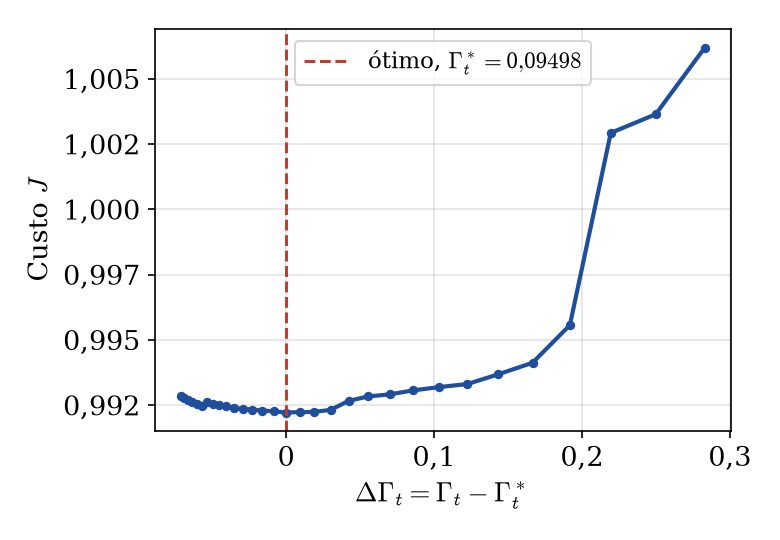
\includegraphics[width=\linewidth]{Desenvolvimento/Otim_sensibilidade_t.png}
    \end{column}
  \end{columns}
  \vspace{0.5em}
  {\small Variação de um ganho de $\Delta\Gamma$ em torno do ótimo
   $\Gamma^*$, com os demais fixos (hélice APC 17x10E).}
  \fonte
\end{frame}

\begin{frame}{Simulação: rotação e torque, hélice APC 15x6E}
  \centering
  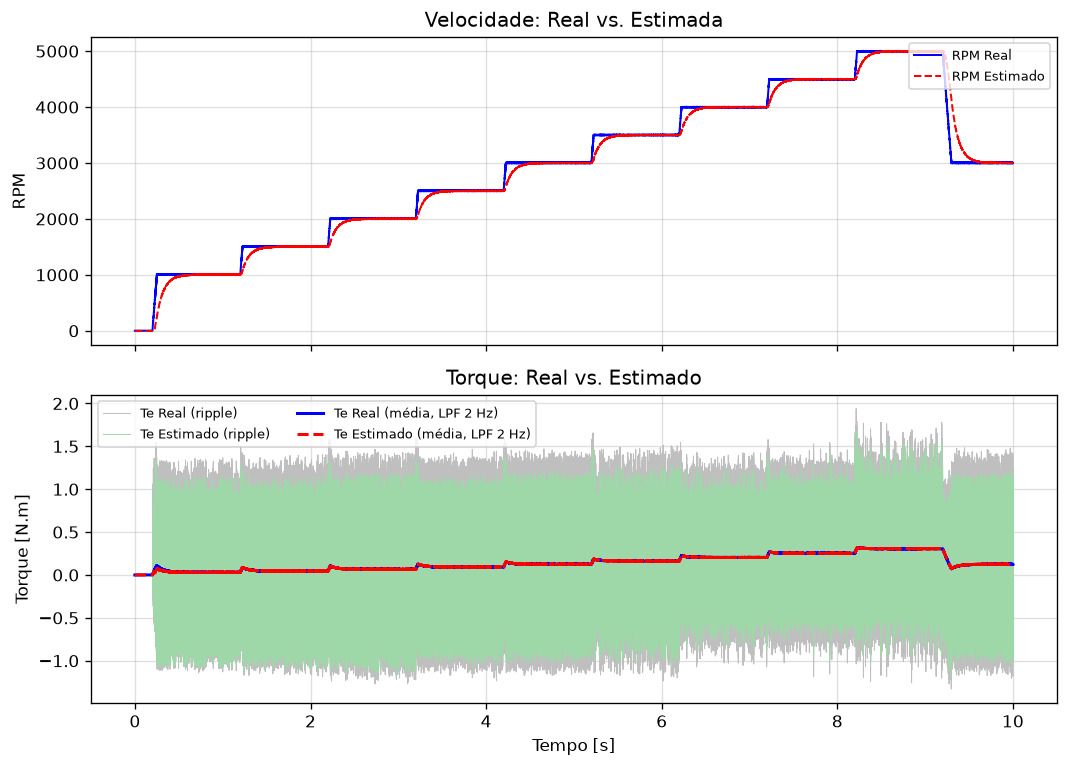
\includegraphics[width=\linewidth,height=0.75\textheight,keepaspectratio]{Desenvolvimento/Torque_rpm_15x6E.png}
  \fonte
\end{frame}

\begin{frame}{Simulação: rotação e torque, hélice APC 17x10E}
  \centering
  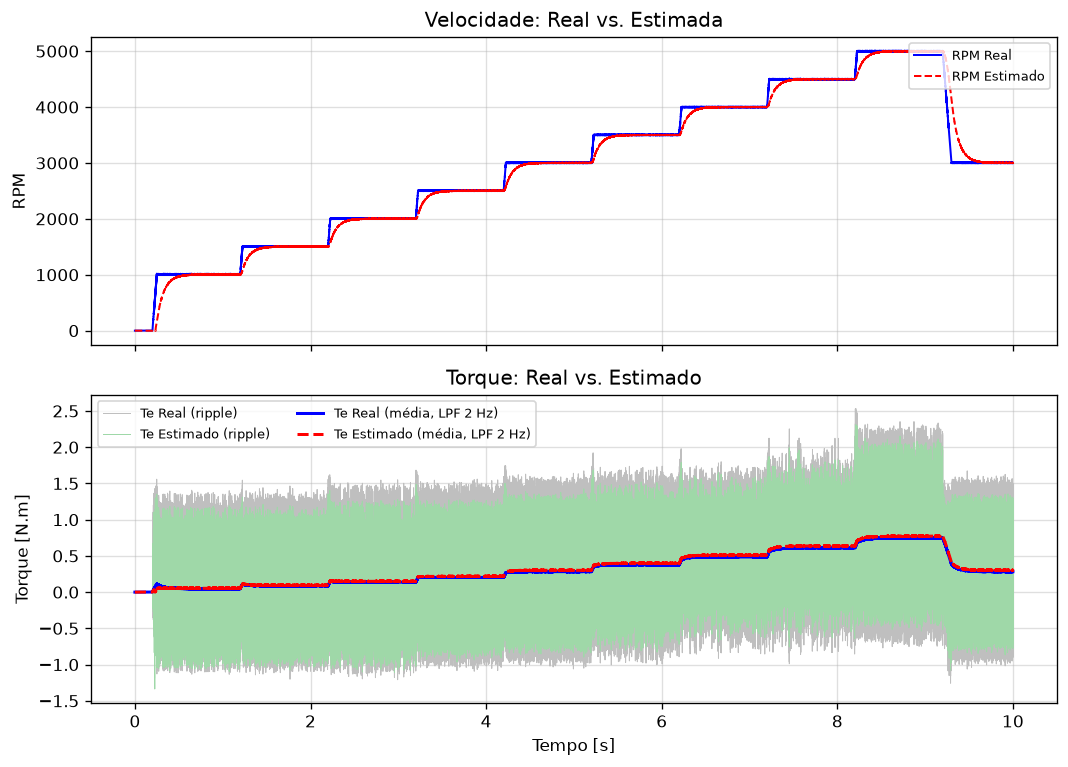
\includegraphics[width=\linewidth,height=0.75\textheight,keepaspectratio]{Desenvolvimento/Torque_rpm_17x10E.png}
  \fonte
\end{frame}

\begin{frame}{Simulação: correntes e FEM nos eixos $\alpha\beta$ (APC 17x10E)}
  \centering
  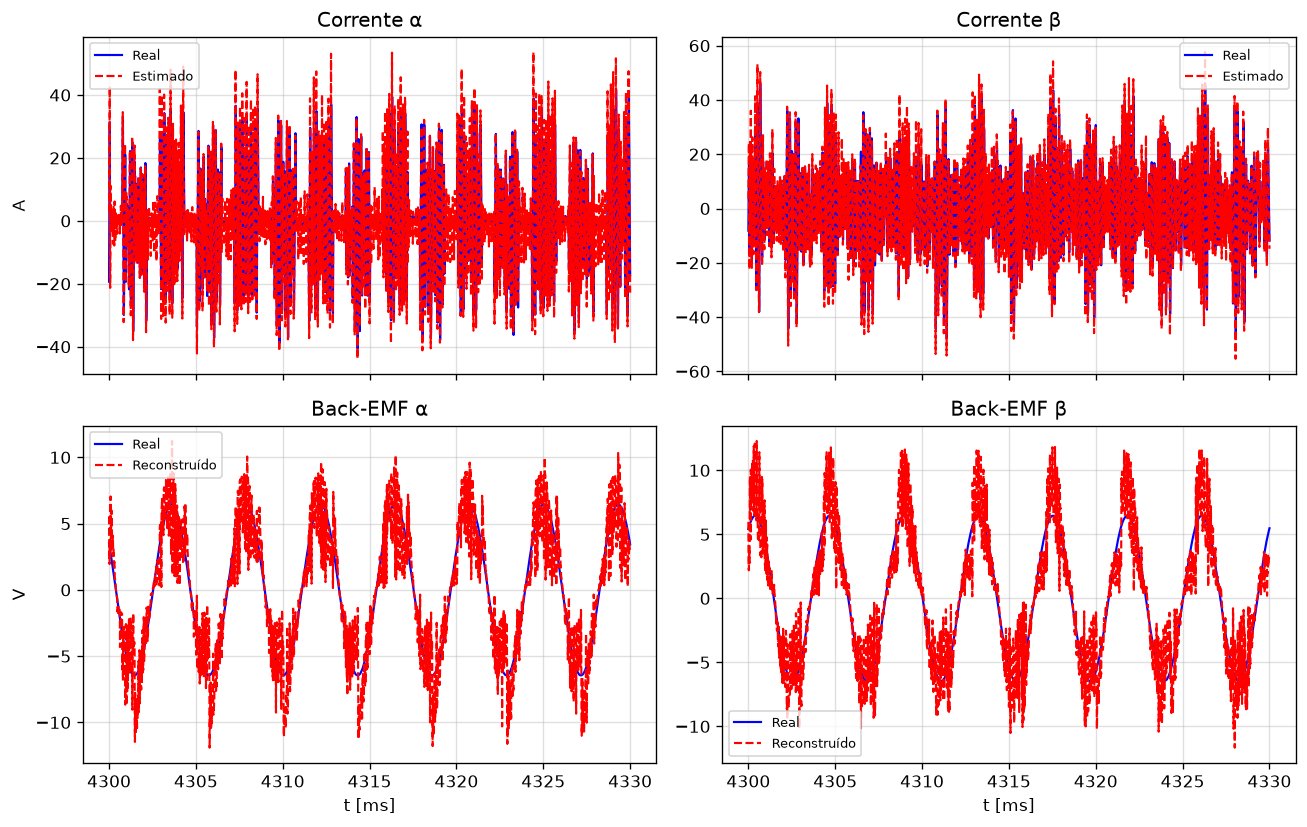
\includegraphics[width=\linewidth,height=0.75\textheight,keepaspectratio]{Desenvolvimento/Eixo_alpha_beta.png}
  \fonte
\end{frame}

\begin{frame}{Simulação: identificação do coeficiente $k_Q$ por patamar}
  \centering
  \begin{fundobranco}
  \begin{tabular}{ccccc}
    \toprule
    & \multicolumn{2}{c}{\textbf{APC 15x6E}} & \multicolumn{2}{c}{\textbf{APC 17x10E}} \\
    \cmidrule(lr){2-3} \cmidrule(lr){4-5}
    \textbf{RPM} &
    \textbf{$\bar{T}$ real / est. [\si{\newton\meter}]} &
    \textbf{$k_{Q}$ real / est. [$10^{-6}$]} &
    \textbf{$\bar{T}$ real / est. [\si{\newton\meter}]} &
    \textbf{$k_{Q}$ real / est. [$10^{-6}$]} \\
    \midrule
    1500 & \num{0,0452} / \num{0,0451} & \num{0,995} / \num{0,998} & \num{0,0850} / \num{0,0848} & \num{2,60} / \num{2,61} \\
    2000 & \num{0,0660} / \num{0,0659} & \num{0,995} / \num{0,997} & \num{0,1365} / \num{0,1365} & \num{2,60} / \num{2,61} \\
    2500 & \num{0,0924} / \num{0,0922} & \num{0,998} / \num{0,998} & \num{0,2022} / \num{0,2019} & \num{2,60} / \num{2,60} \\
    3000 & \num{0,1242} / \num{0,1243} & \num{0,998} / \num{1,00}  & \num{0,2823} / \num{0,2820} & \num{2,60} / \num{2,60} \\
    3500 & \num{0,1616} / \num{0,1612} & \num{0,999} / \num{0,999} & \num{0,3767} / \num{0,3756} & \num{2,60} / \num{2,60} \\
    4000 & \num{0,2042} / \num{0,2041} & \num{0,998} / \num{1,00}  & \num{0,4851} / \num{0,4841} & \num{2,60} / \num{2,60} \\
    4500 & \num{0,2527} / \num{0,2521} & \num{1,00} / \num{0,999}  & \num{0,6079} / \num{0,6064} & \num{2,60} / \num{2,60} \\
    5000 & \num{0,3062} / \num{0,3060} & \num{0,999} / \num{1,00}  & \num{0,7450} / \num{0,7380} & \num{2,60} / \num{2,58} \\
    3000\textsuperscript{a} & \num{0,1243} / \num{0,1241} & \num{0,998} / \num{0,968} & \num{0,2823} / \num{0,2824} & \num{2,60} / \num{2,52} \\
    \midrule
    \textbf{Est./nom.} & \multicolumn{2}{c}{\num{0,996} / \num{1,00} (\SI{0,45}{\percent})} &
        \multicolumn{2}{c}{\num{2,59} / \num{2,60} (\SI{0,32}{\percent})} \\
    \bottomrule
    \multicolumn{5}{l}{\textsuperscript{a} Patamar após a desaceleração de \SIrange{5000}{3000}{RPM}.}
  \end{tabular}
  \end{fundobranco}
  \fonte
\end{frame}

%% --- laboratório com osciloscópio ----------------------------------
\begin{frame}{Ensaio em laboratório com osciloscópio}
  \begin{columns}[c]
    \begin{column}{0.55\textwidth}
      \centering
      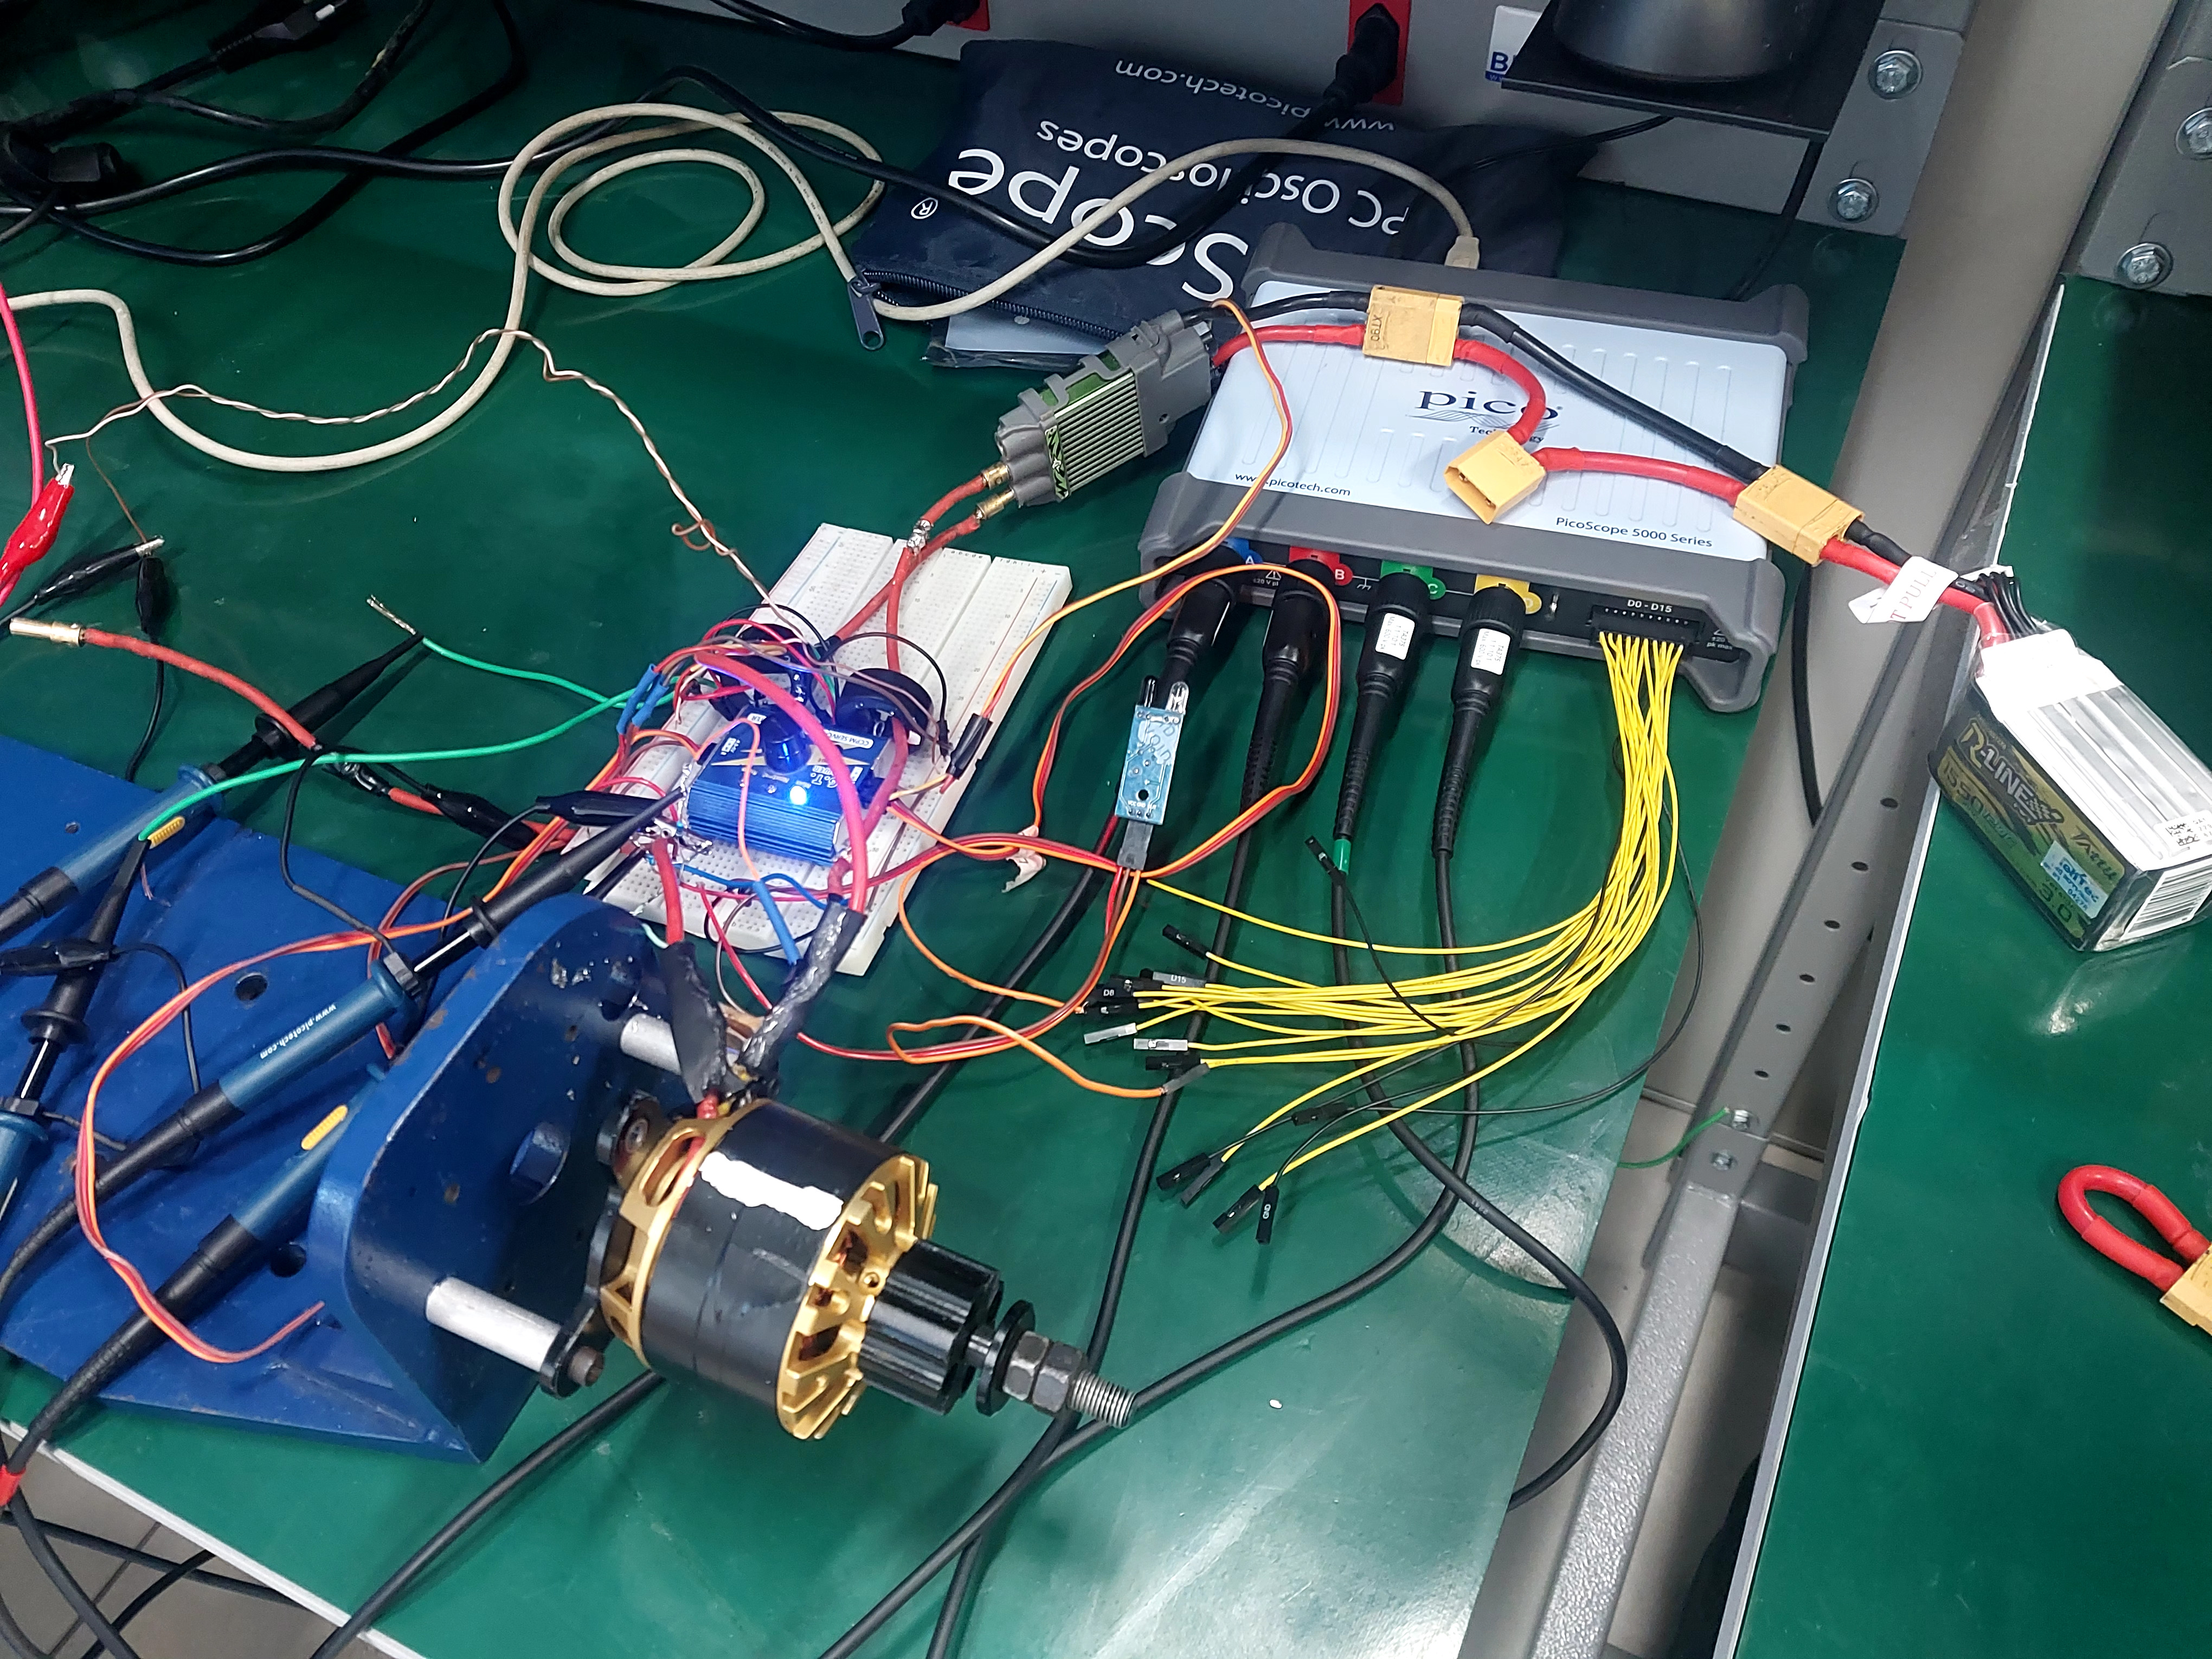
\includegraphics[width=\linewidth,height=0.72\textheight,keepaspectratio]{Resultados/ensaio_motor_vazio.jpg}
    \end{column}
    \begin{column}{0.45\textwidth}
      \begin{itemize}
        \small
        \item PicoScope Série 5000, laboratório do PET
        \item 4 canais analógicos: duas tensões e duas correntes de fase
              (sensores Hall da placa)
        \item 2 canais digitais: comando do acelerador e tacômetro óptico
        \item Terceira fase pela soma nula
        \item Neutro virtual com três resistores
        \item Dois controladores: Castle Talon \SI{90}{\ampere} e Flycolor
              \SI{150}{\ampere}
      \end{itemize}
    \end{column}
  \end{columns}
  \fonte[Autor (2026); Nidec Corporation ({[\textit{s. d.}]})]
\end{frame}

\begin{frame}{Laboratório: perdas a vazio}
  \centering
  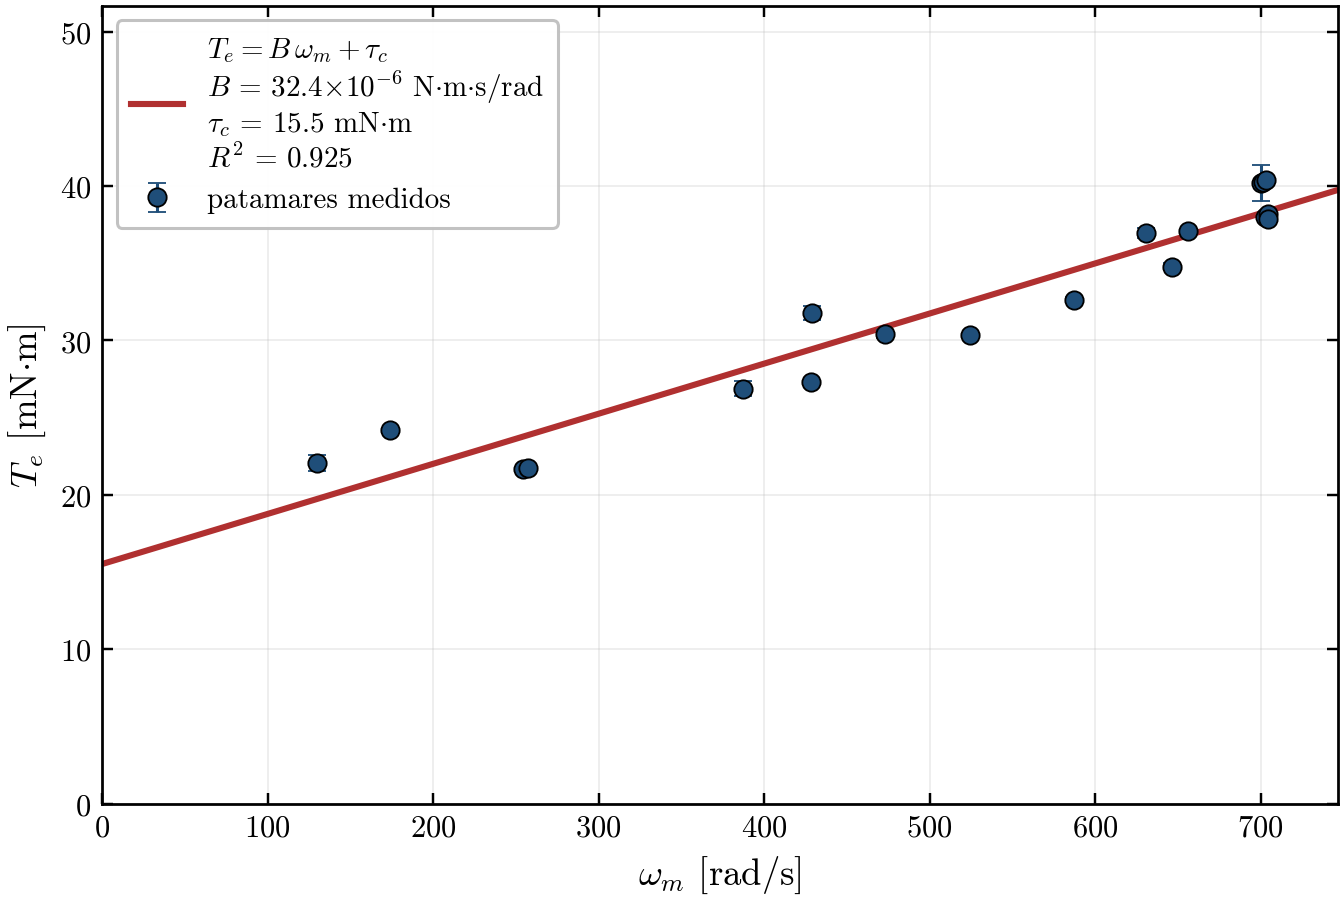
\includegraphics[width=\linewidth,height=0.75\textheight,keepaspectratio]{Resultados/bancada_te_omega.png}
  \fonte
\end{frame}

\begin{frame}{Laboratório: observador nos registros do osciloscópio}
  \begin{columns}[c]
    \begin{column}{0.58\textwidth}
      \centering
      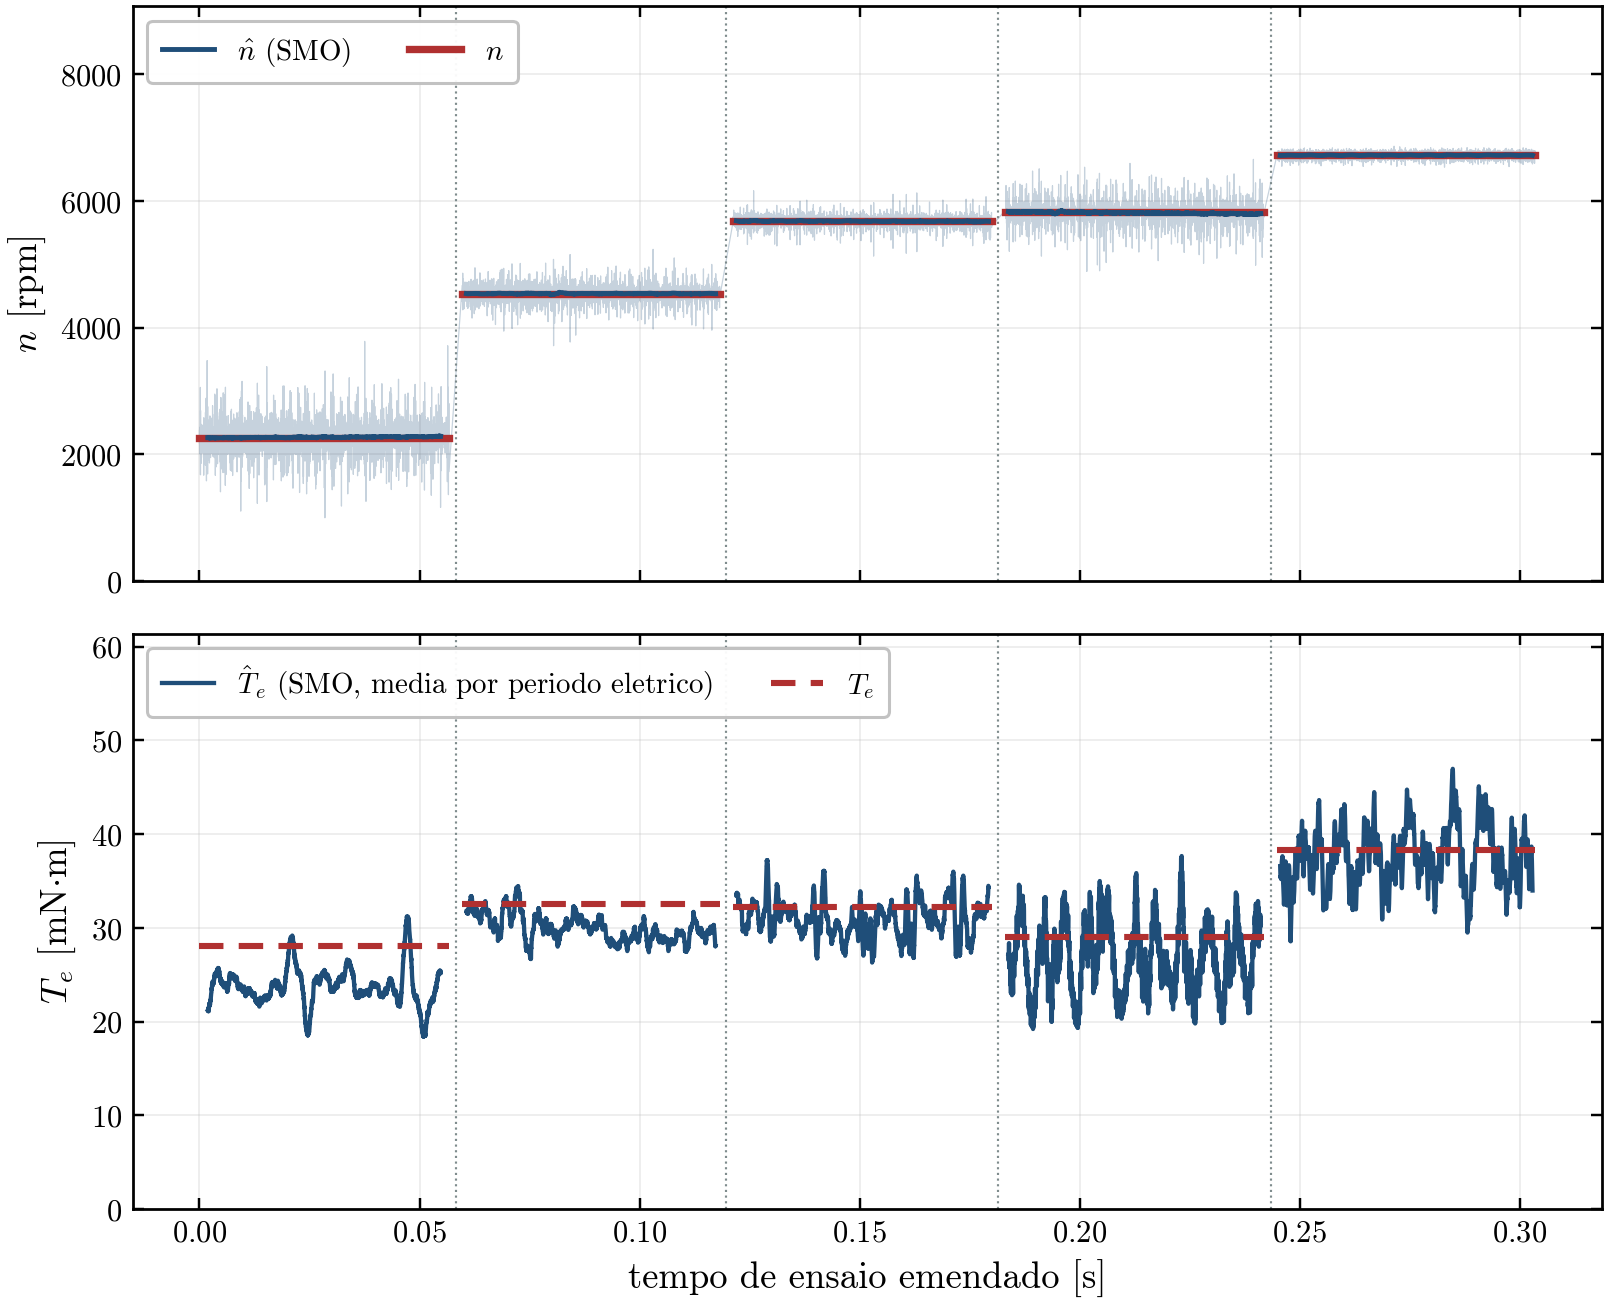
\includegraphics[width=\linewidth,height=0.72\textheight,keepaspectratio]{Resultados/bancada_smo_rpm_torque.png}
    \end{column}
    \begin{column}{0.42\textwidth}
      \begin{itemize}
        \small
        \item Rotação: erro médio de \SI{0,092}{\percent} contra o
              tacômetro
        \item Ângulo: \SI{0,3}{\degree} de diferença média contra a
              integral dos pulsos
        \item Torque: \SI{-7,2}{\percent} contra o balanço de potência
        \item Abaixo de cerca de \num{1930} RPM o ângulo não trava: rotação
              disponível, torque não
      \end{itemize}
    \end{column}
  \end{columns}
  \fonte
\end{frame}

%% --- sistema de aquisição e hélices --------------------------------
\begin{frame}{Sistema de aquisição montado}
  \begin{columns}[t]
    \begin{column}{0.33\textwidth}
      \centering
      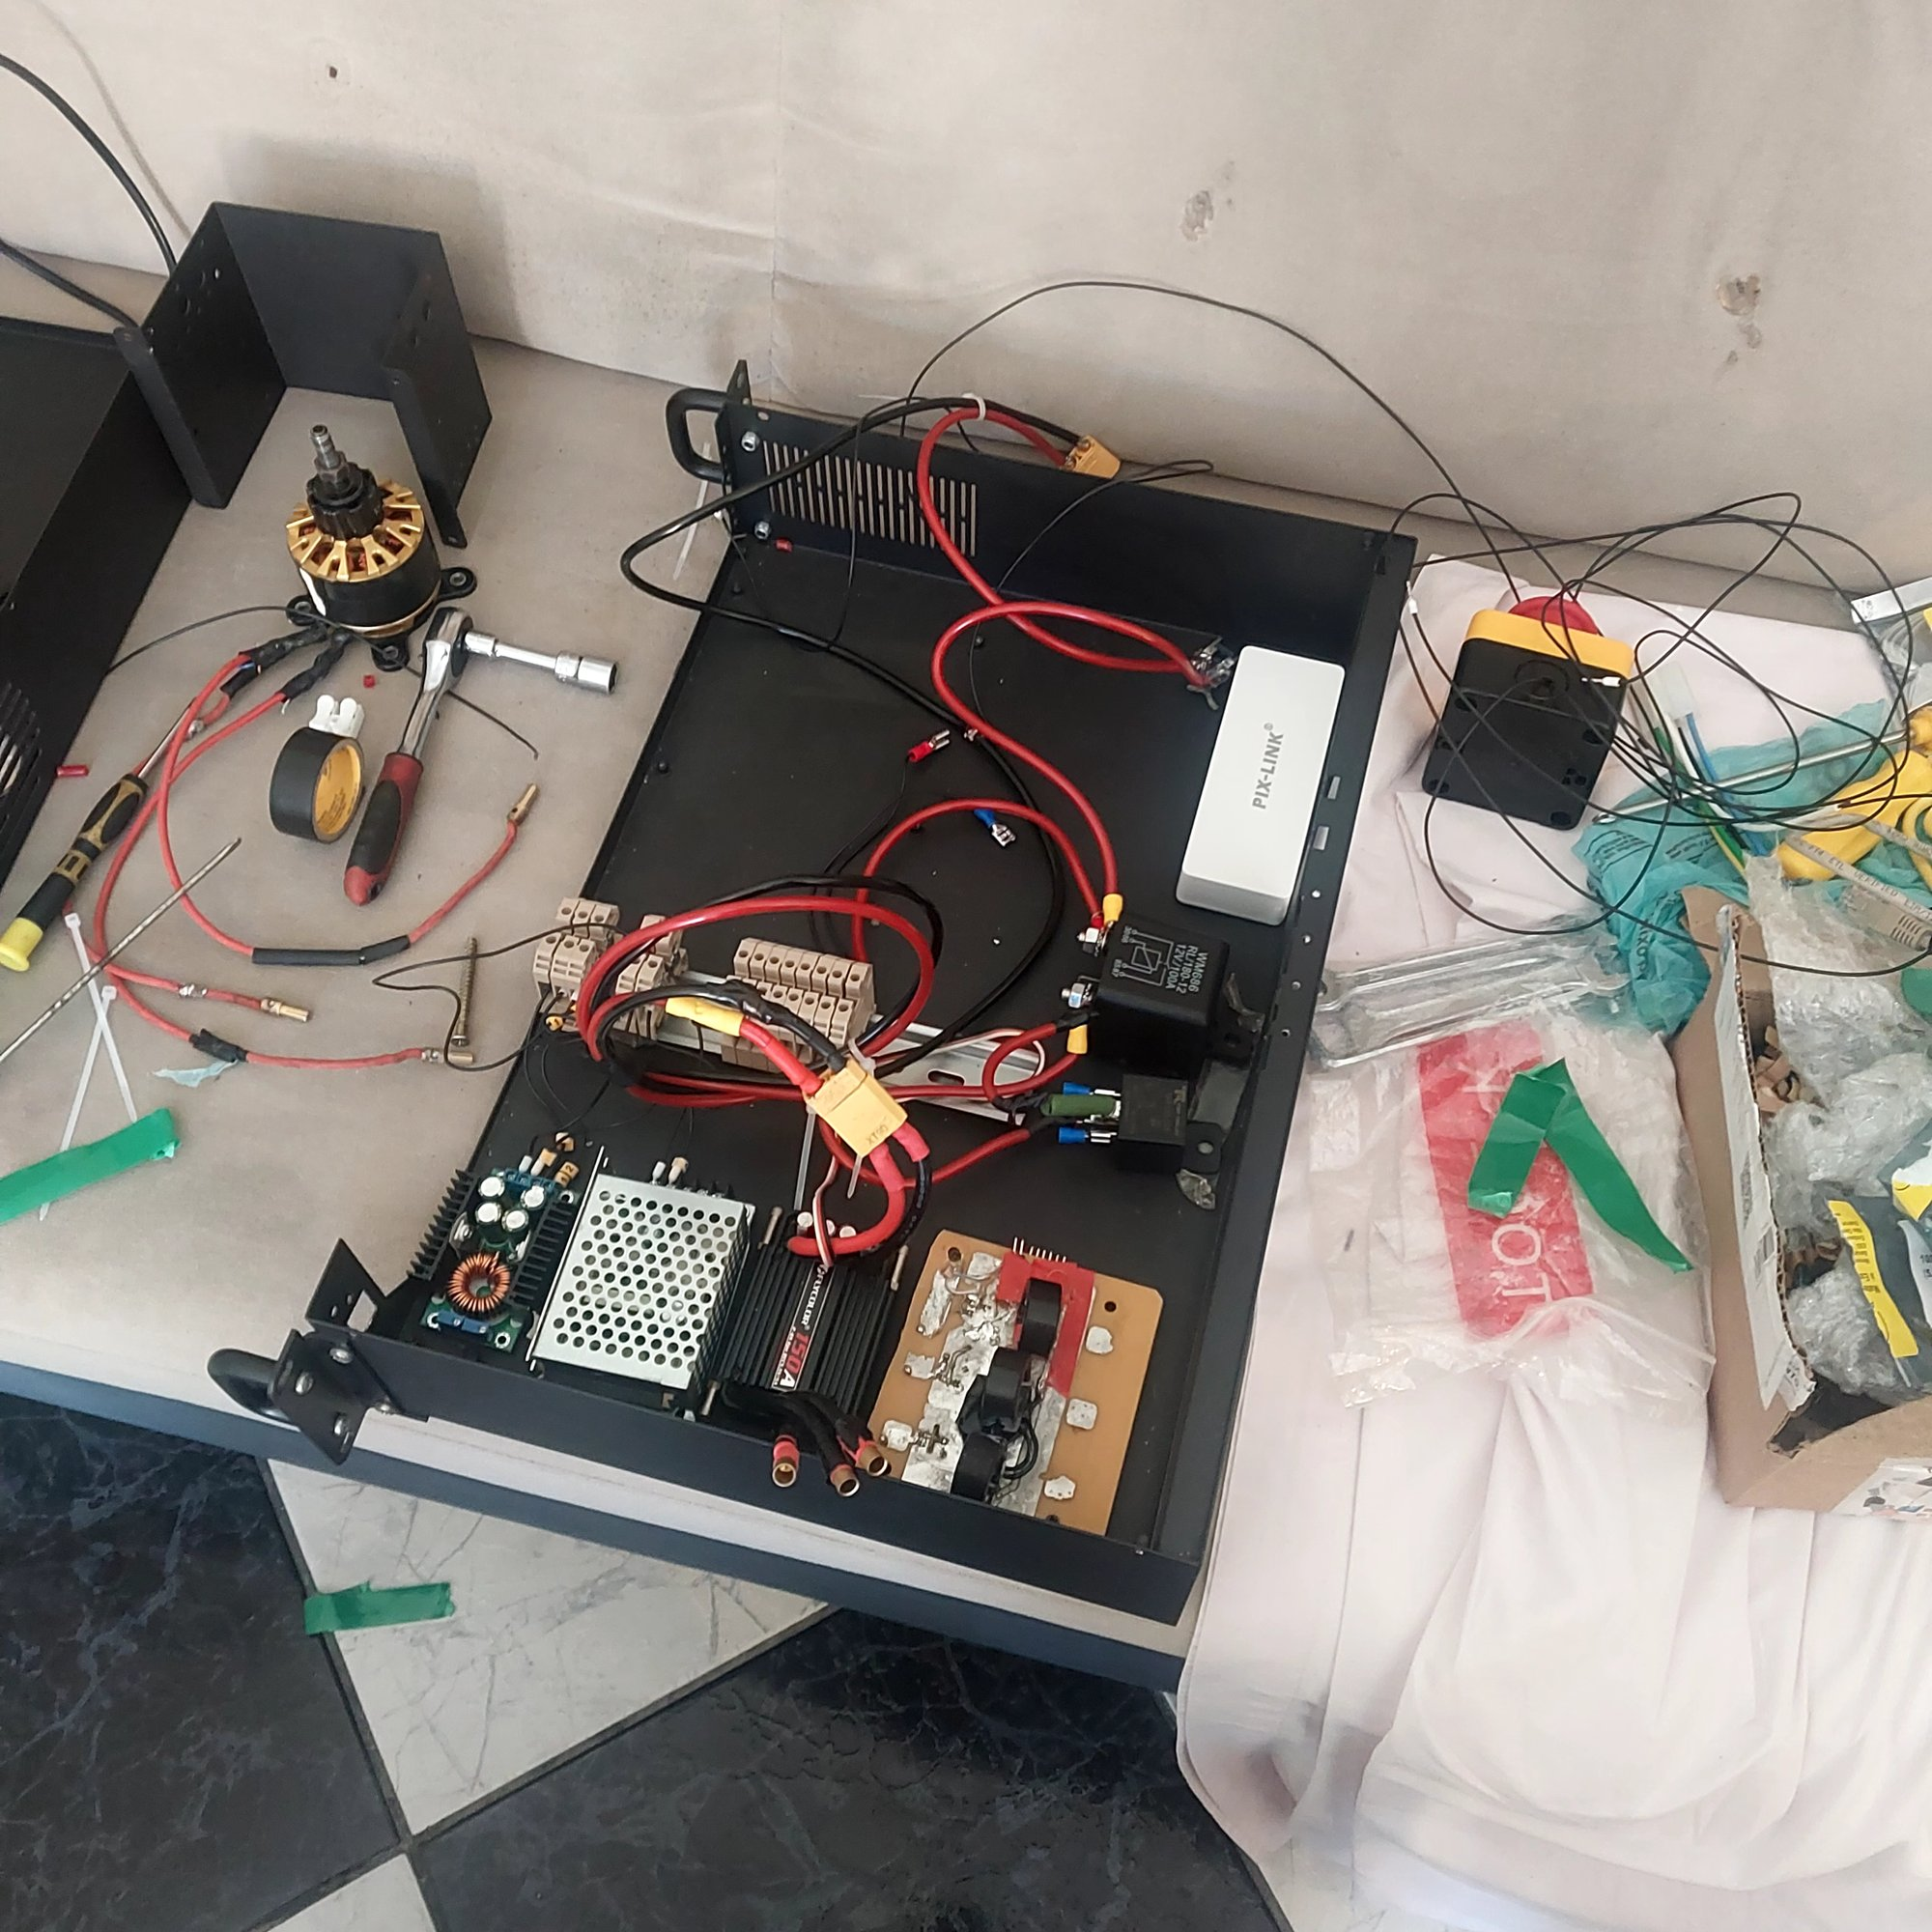
\includegraphics[width=\linewidth,height=0.68\textheight,keepaspectratio]{Resultados/processo montagem.jpg}\\[0.3em]
      {\small Parte de potência}
    \end{column}
    \begin{column}{0.33\textwidth}
      \centering
      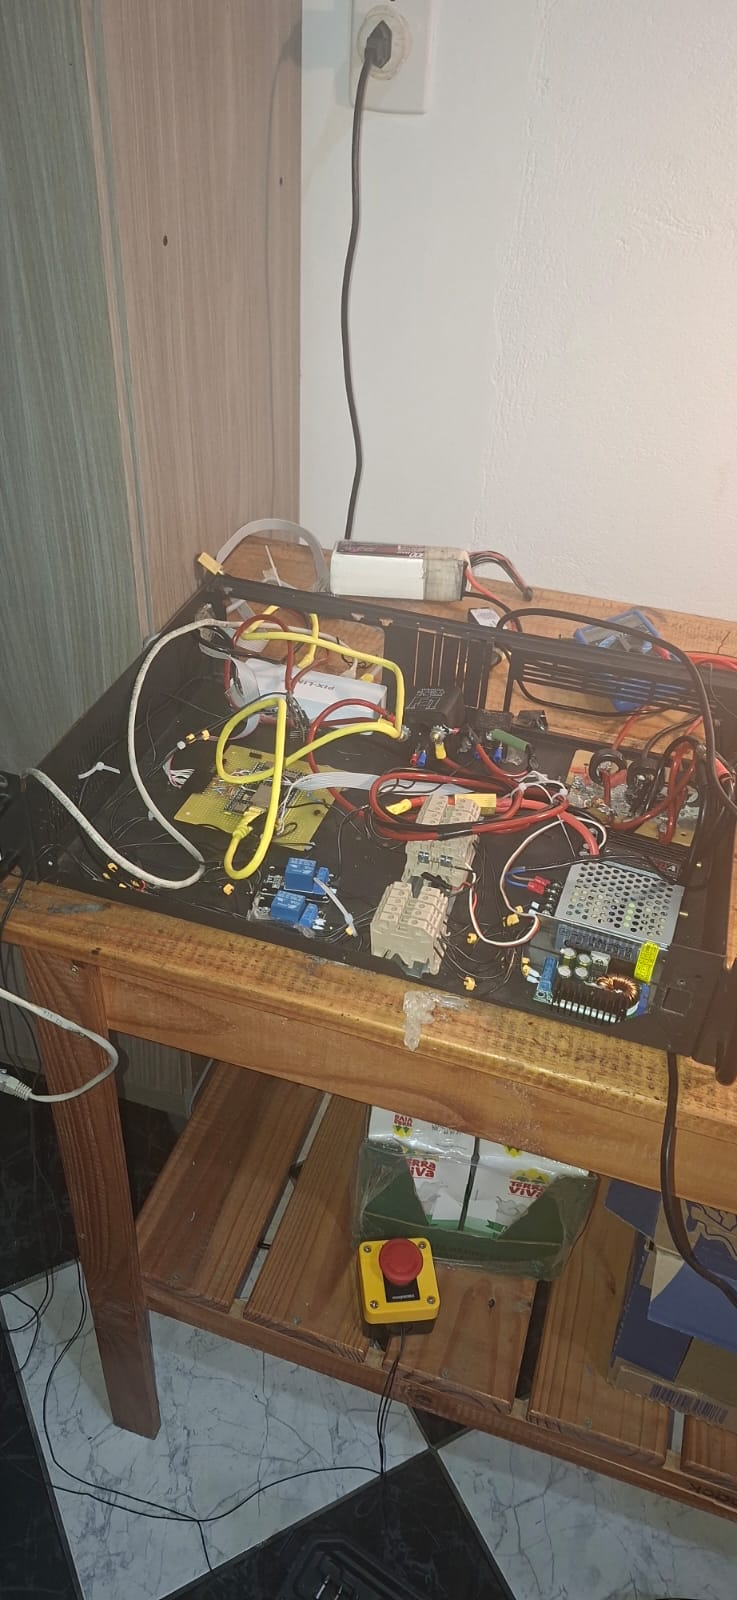
\includegraphics[width=\linewidth,height=0.68\textheight,keepaspectratio]{Resultados/montagem finalizada.jpeg}\\[0.3em]
      {\small Fiação concluída}
    \end{column}
    \begin{column}{0.33\textwidth}
      \centering
      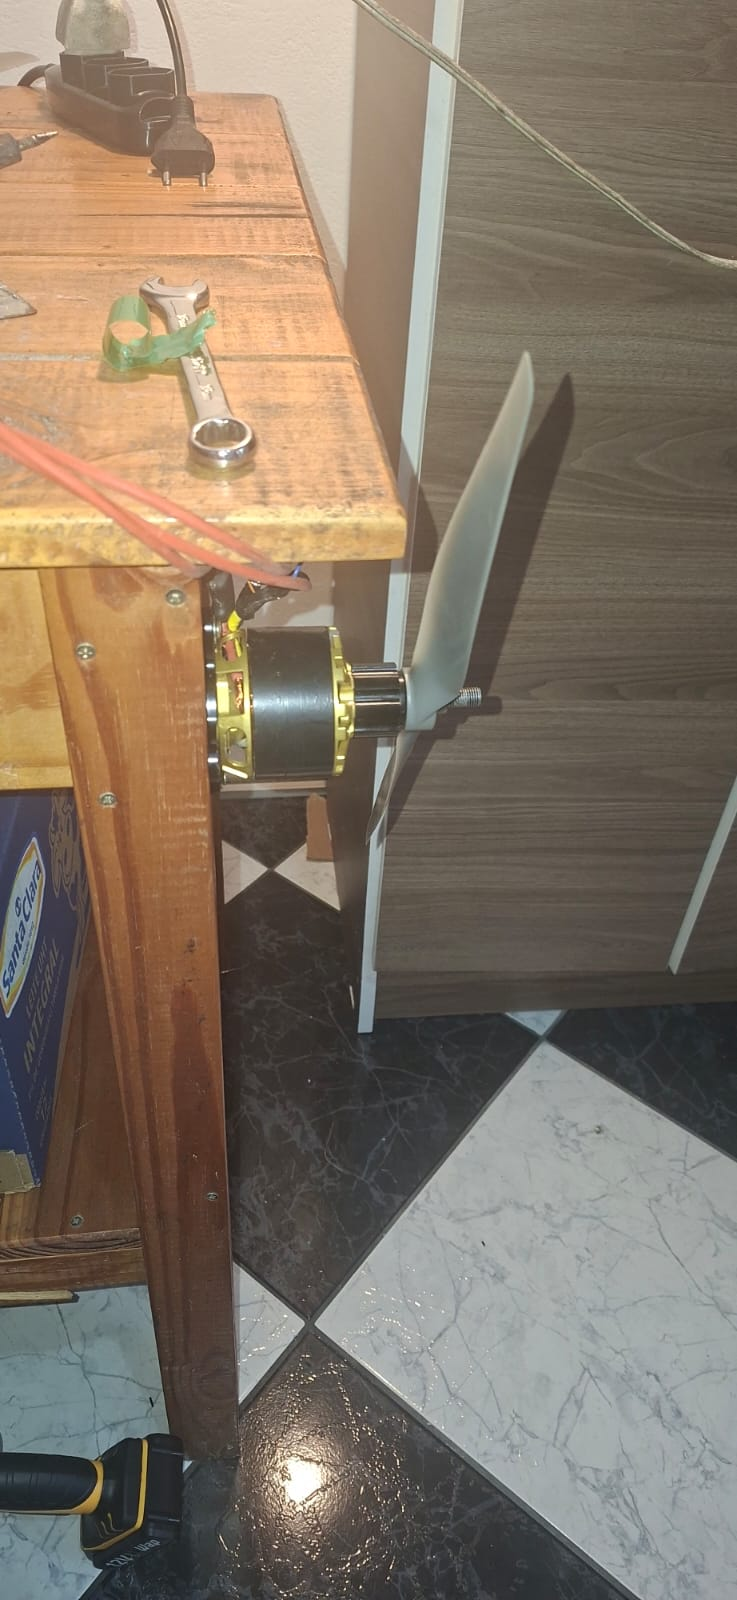
\includegraphics[width=\linewidth,height=0.68\textheight,keepaspectratio]{Resultados/montagem_motor.jpeg}\\[0.3em]
      {\small Motor e hélice na mesa}
    \end{column}
  \end{columns}
  \centering
  \fonte
\end{frame}

\begin{frame}{Ensaio na interface: hélice APC 15x6E}
  \centering
  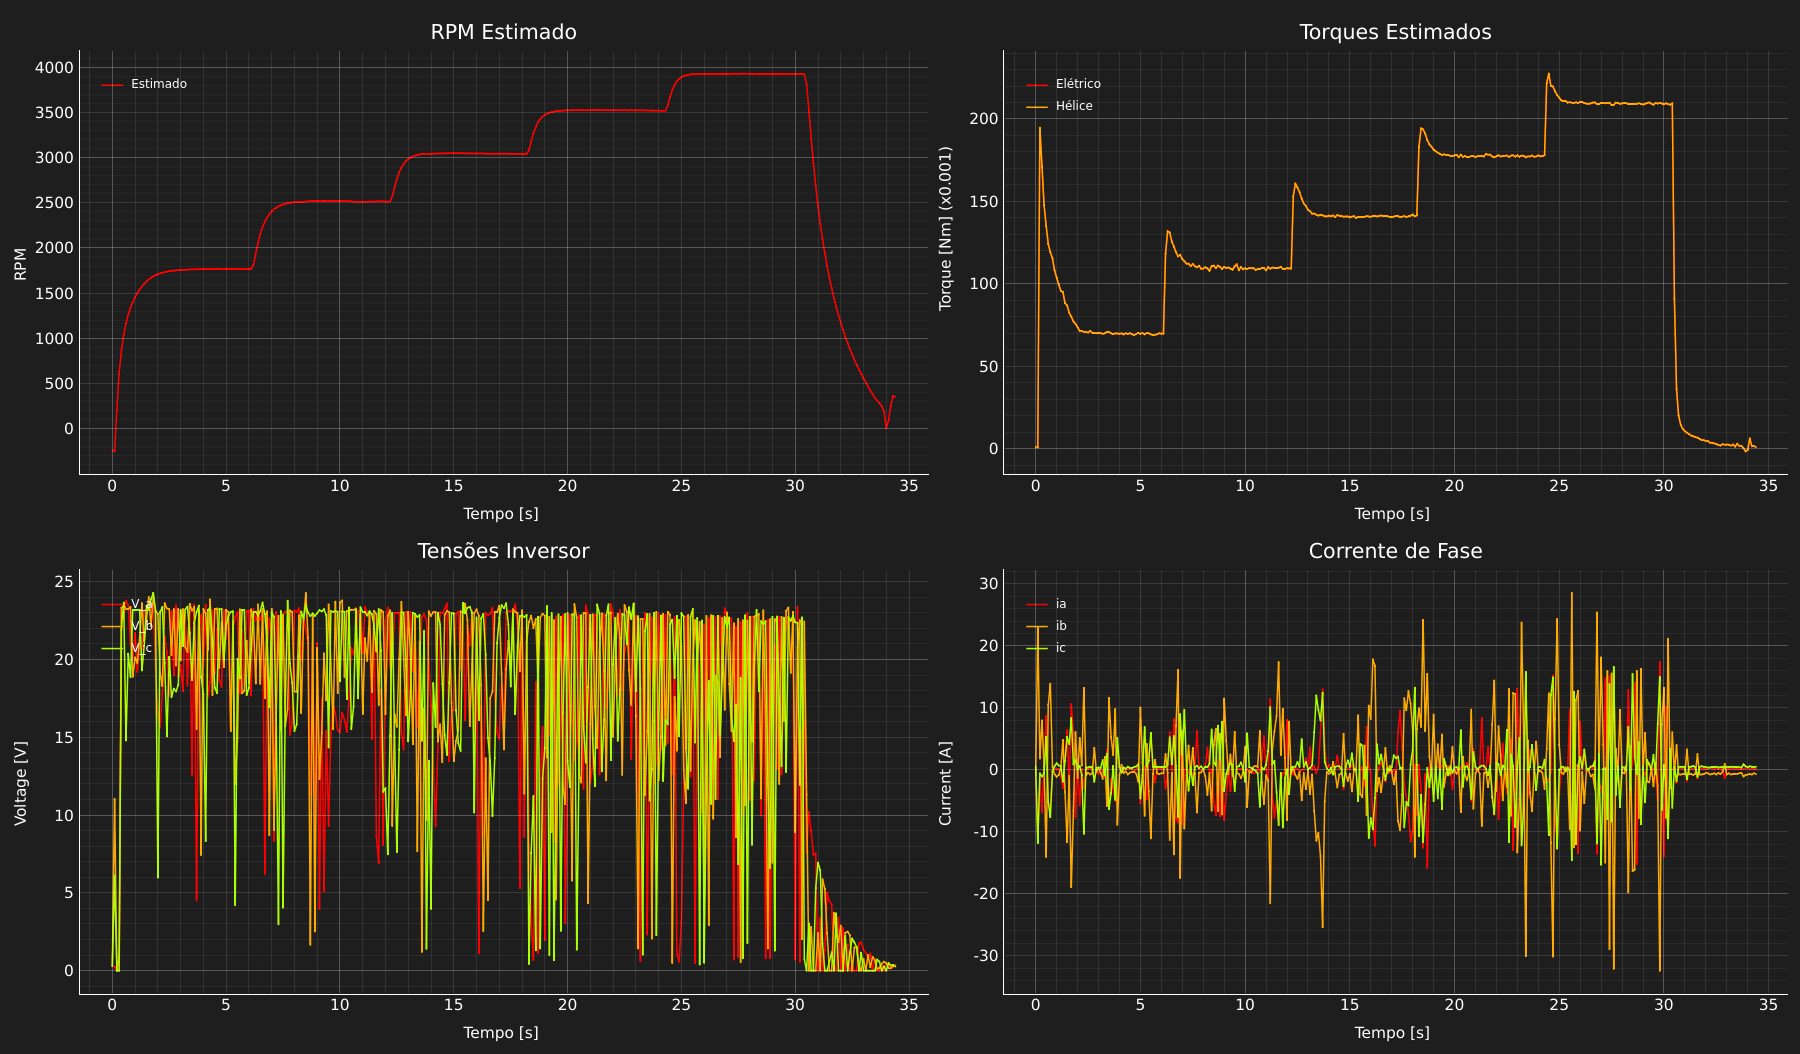
\includegraphics[width=\linewidth,height=0.75\textheight,keepaspectratio]{Resultados/helice/gui_ensaio_15x6E.png}
  \fonte
\end{frame}

\begin{frame}{Ensaio na interface: hélice APC 17x10E}
  \centering
  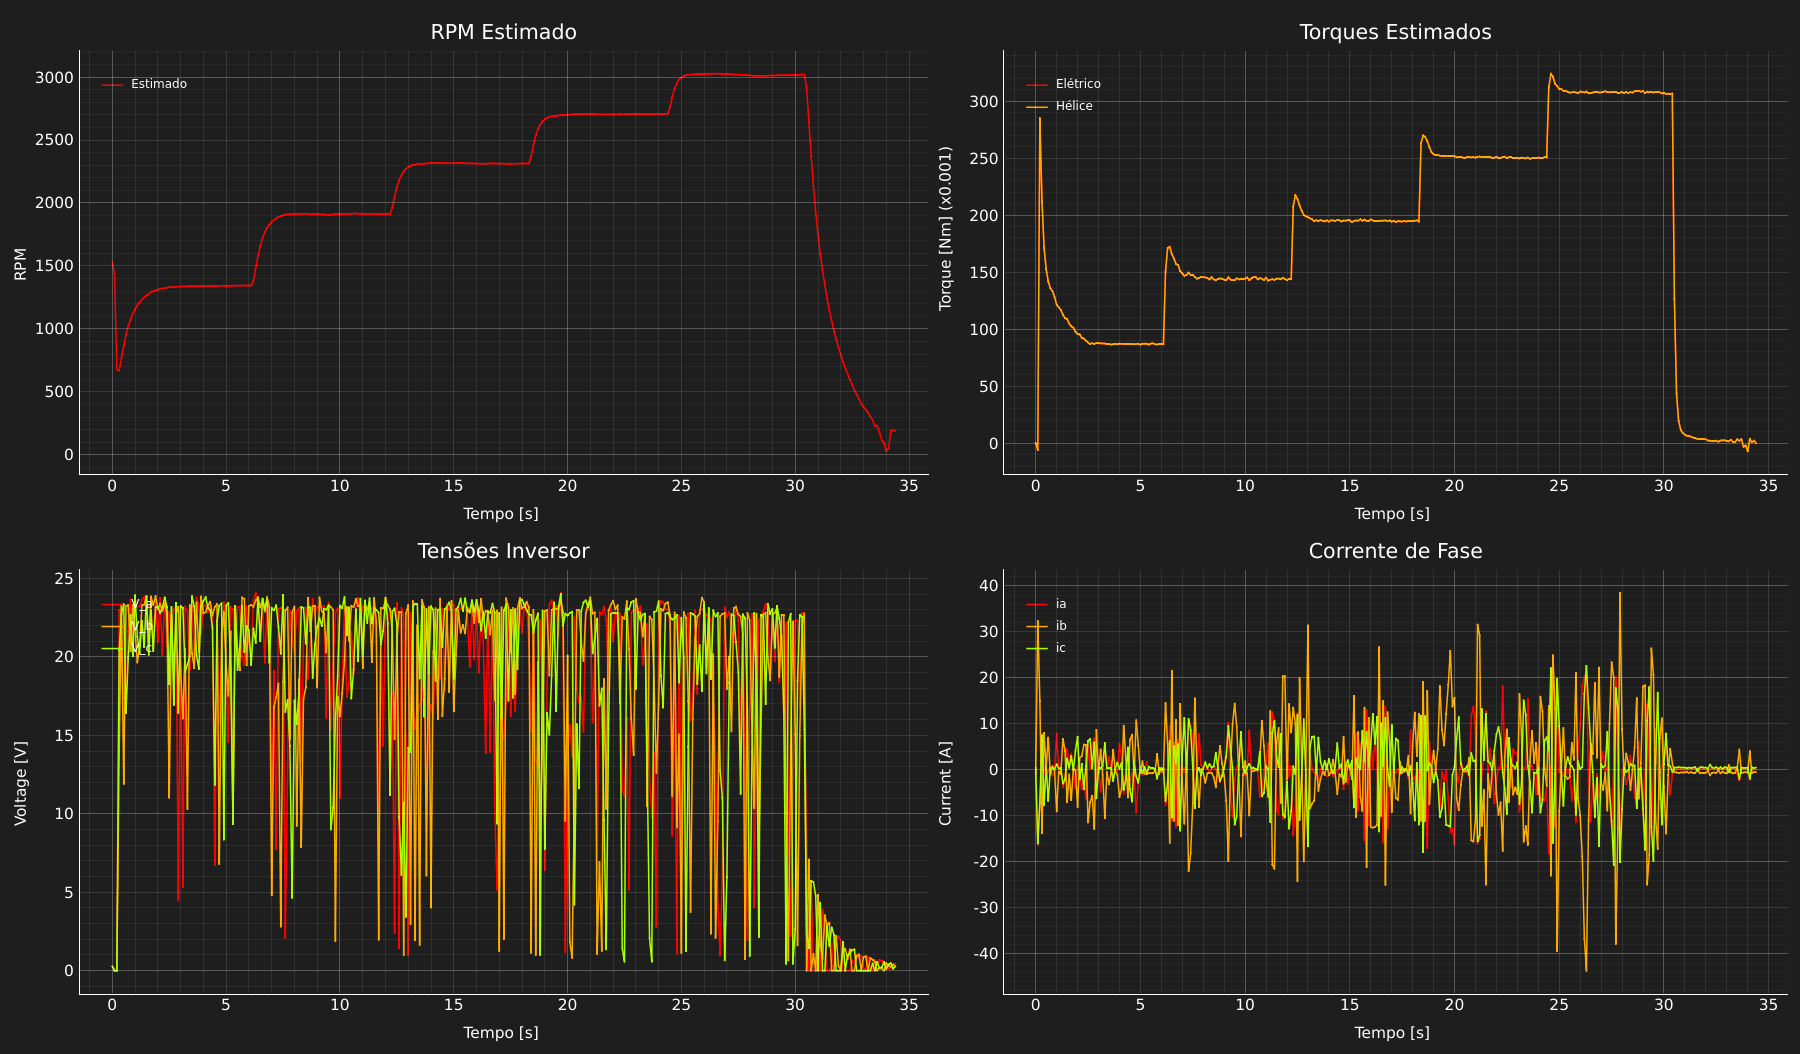
\includegraphics[width=\linewidth,height=0.75\textheight,keepaspectratio]{Resultados/helice/gui_ensaio_17x10E.png}
  \fonte
\end{frame}

\pgfplotsset{
  helslide/.style={width=7cm, height=5.4cm, grid=both,
    grid style={dotted,gray!40}, xmin=1000, xmax=4000, xtick distance=1000,
    xlabel={Rotação [RPM]}, ylabel={$C_Q$},
    tick label style={font=\scriptsize}, label style={font=\small},
    title style={font=\small},
    scaled x ticks=false, scaled y ticks=false,
    xticklabel style={/pgf/number format/1000 sep={}},
    yticklabel style={/pgf/number format/fixed,
                      /pgf/number format/precision=4,
                      /pgf/number format/use comma},
    legend style={at={(0.5,-0.3)}, anchor=north, legend columns=3,
                  font=\scriptsize}},
  hsel/.style={table/comment chars={\#}},
}
% perdas descontadas: 1º ensaio (laboratório) e 2º ensaio (sistema)
\newcommand{\perdasum}{(32.4e-6*\thisrow{rpm}*0.1047198 + 15.5e-3)}
\newcommand{\perdasdois}{(1.0116e-04*\thisrow{rpm}*0.1047198 + 2.0713e-02)}
% \cqpainel{hélice}{D^5}{ymin}{ymax}{cor}{marca 1º}{marca 2º}{mostra 2º: 0/1}
\newcommand{\cqpainel}[8]{%
  \begin{tikzpicture}
  \begin{axis}[helslide, title={APC #1}, ymin=#3, ymax=#4]
    \addplot[thick, #5, restrict x to domain=1000:4000]
      table[x=rpm, y=CQ] {\dadoshelice/apc_#1_estatico.dat};
    \addlegendentry{APC}
    \addplot[only marks, mark=#6, #5, mark size=2.5pt]
      table[hsel, x=rpm, y expr={(\thisrow{Te_Nm} - \perdasum) / (\thisrow{rho}*(\thisrow{rpm}/60)^2*#2)}]
      {\dadoshelice/medido_#1.dat};
    \addlegendentry{1º ensaio}
    \ifnum#8=1
    \addplot[only marks, mark=#7, #5, mark size=2.5pt]
      table[hsel, x=rpm, y expr={(\thisrow{Te_Nm} - \perdasdois) / (\thisrow{rho}*(\thisrow{rpm}/60)^2*#2)}]
      {\dadoshelice/medido_repeticao_#1.dat};
    \addlegendentry{2º ensaio}
    \fi
  \end{axis}
  \end{tikzpicture}}

\begin{frame}{1º ensaio: coeficiente de torque das hélices}
  \centering
  \begin{fundobranco}
    \cqpainel{15x6E}{8.0283e-3}{0.003}{0.0068}{blue!65!black}{o}{*}{0}\hspace{0.8cm}%
    \cqpainel{17x10E}{1.50111e-2}{0.0045}{0.0085}{red!65!black}{square}{square*}{0}
  \end{fundobranco}
  \fonte[Autor (2026); adaptado de APC Propellers (2026)]
\end{frame}

\begin{frame}{1º ensaio: torque das hélices}
  \centering
  \begin{fundobranco}
  \begin{tabular}{cccccc}
    \toprule
    \textbf{Hélice} & \textbf{Acelerador} & \textbf{Rotação [RPM]} &
    \textbf{$Q$ teórico [\si{\newton\meter}]} &
    \textbf{$Q$ bancada [\si{\newton\meter}]} & \textbf{Erro} \\
    \midrule
    15x6E  & \SI{20}{\percent} & \num{1770} & \num{0,0343} & \num{0,0504} & \SI{+47,0}{\percent} \\
           & \SI{30}{\percent} & \num{3050} & \num{0,0949} & \num{0,1191} & \SI{+25,5}{\percent} \\
           & \SI{40}{\percent} & \num{3937} & \num{0,1540} & \num{0,1862} & \SI{+21,0}{\percent} \\
    \midrule
    17x10E & \SI{20}{\percent} & \num{1335} & \num{0,0520} & \num{0,0688} & \SI{+32,3}{\percent} \\
           & \SI{30}{\percent} & \num{2308} & \num{0,1462} & \num{0,1758} & \SI{+20,3}{\percent} \\
           & \SI{40}{\percent} & \num{3010} & \num{0,2429} & \num{0,2888} & \SI{+18,9}{\percent} \\
    \bottomrule
  \end{tabular}
  \end{fundobranco}
  \fonte[Autor (2026); teórico adaptado de APC Propellers (2026)]
\end{frame}

\begin{frame}{Perdas a vazio: 1º e 2º ensaio}
  \centering
  \begin{fundobranco}
  \begin{tikzpicture}
  \begin{axis}[width=11cm, height=6cm, grid=both,
      grid style={dotted,gray!40}, xmin=2300, xmax=6500, ymin=0.02, ymax=0.1,
      xlabel={Rotação [RPM]}, ylabel={Torque de perdas [\si{\newton\meter}]},
      tick label style={font=\scriptsize}, label style={font=\small},
      scaled x ticks=false, xticklabel style={/pgf/number format/1000 sep={}},
      yticklabel style={/pgf/number format/fixed, /pgf/number format/precision=2,
                        /pgf/number format/use comma},
      legend style={at={(0.5,-0.25)}, anchor=north, legend columns=3, font=\scriptsize}]
    \addplot[only marks, mark=*, mark size=2pt, blue!75!black,
             error bars/.cd, y dir=both, y explicit]
      table[x=rpm, y=Te_Nm, y error=Te_err, comment chars={\#}] {\dadoshelice/vazio_perdas.dat};
    \addlegendentry{patamares a vazio (2º ensaio)}
    \addplot[very thick, blue!75!black, domain=2300:6500, samples=2]
      {1.0116e-04*x*0.1047198 + 2.0713e-02};
    \addlegendentry{ajuste linear (2º ensaio)}
    \addplot[very thick, dashed, red!80!black, domain=2300:6500, samples=2]
      {32.4e-6*x*0.1047198 + 15.5e-3};
    \addlegendentry{perdas do 1º ensaio}
  \end{axis}
  \end{tikzpicture}
  \end{fundobranco}
  \fonte
\end{frame}

\begin{frame}{2º ensaio: coeficiente de torque das hélices}
  \centering
  \begin{fundobranco}
    \cqpainel{15x6E}{8.0283e-3}{0.003}{0.0068}{blue!65!black}{o}{*}{1}\hspace{0.8cm}%
    \cqpainel{17x10E}{1.50111e-2}{0.0045}{0.0085}{red!65!black}{square}{square*}{1}
  \end{fundobranco}
  \fonte[Autor (2026); adaptado de APC Propellers (2026)]
\end{frame}

\begin{frame}{2º ensaio: hélice APC 15x6E}
  \centering
  \begin{fundobranco}
  \begin{tabular}{ccccccc}
    \toprule
    & & \multicolumn{2}{c}{\textbf{$Q$ [\si{\newton\meter}]}} & \multicolumn{2}{c}{\textbf{$C_Q$}} & \\
    \cmidrule(lr){3-4}\cmidrule(lr){5-6}
    \textbf{Acelerador} & \textbf{Rotação [RPM]} & \textbf{Teórico} & \textbf{Bancada} & \textbf{Teórico} & \textbf{Bancada} & \textbf{Erro} \\
    \midrule
    \SI{20}{\percent} & \num{1759} & \num{0,0339} & \num{0,0329} $\pm$ \num{0,0025} & \num{0,00404} & \num{0,00390} $\pm$ \num{0,00030} & \SI{-2,8}{\percent} \\
    \SI{25}{\percent} & \num{2516} & \num{0,0661} & \num{0,0657} $\pm$ \num{0,0036} & \num{0,00383} & \num{0,00380} $\pm$ \num{0,00022} & \SI{-0,5}{\percent} \\
    \SI{30}{\percent} & \num{3046} & \num{0,0947} & \num{0,0925} $\pm$ \num{0,0044} & \num{0,00373} & \num{0,00365} $\pm$ \num{0,00019} & \SI{-2,3}{\percent} \\
    \SI{35}{\percent} & \num{3524} & \num{0,1248} & \num{0,1251} $\pm$ \num{0,0055} & \num{0,00368} & \num{0,00369} $\pm$ \num{0,00018} & \SI{+0,2}{\percent} \\
    \SI{40}{\percent} & \num{3927} & \num{0,1533} & \num{0,1537} $\pm$ \num{0,0065} & \num{0,00364} & \num{0,00365} $\pm$ \num{0,00017} & \SI{+0,3}{\percent} \\
    \bottomrule
  \end{tabular}
  \end{fundobranco}
  \fonte[Autor (2026); teórico adaptado de APC Propellers (2026)]
\end{frame}

\begin{frame}{2º ensaio: hélice APC 17x10E}
  \centering
  \begin{fundobranco}
  \begin{tabular}{ccccccc}
    \toprule
    & & \multicolumn{2}{c}{\textbf{$Q$ [\si{\newton\meter}]}} & \multicolumn{2}{c}{\textbf{$C_Q$}} & \\
    \cmidrule(lr){3-4}\cmidrule(lr){5-6}
    \textbf{Acelerador} & \textbf{Rotação [RPM]} & \textbf{Teórico} & \textbf{Bancada} & \textbf{Teórico} & \textbf{Bancada} & \textbf{Erro} \\
    \midrule
    \SI{20}{\percent} & \num{1339} & \num{0,0523} & \num{0,0555} $\pm$ \num{0,0034} & \num{0,00583} & \num{0,00606} $\pm$ \num{0,00039} & \SI{+6,2}{\percent} \\
    \SI{25}{\percent} & \num{1912} & \num{0,1022} & \num{0,1076} $\pm$ \num{0,0046} & \num{0,00556} & \num{0,00576} $\pm$ \num{0,00027} & \SI{+5,3}{\percent} \\
    \SI{30}{\percent} & \num{2314} & \num{0,1469} & \num{0,1560} $\pm$ \num{0,0061} & \num{0,00546} & \num{0,00571} $\pm$ \num{0,00025} & \SI{+6,2}{\percent} \\
    \SI{35}{\percent} & \num{2705} & \num{0,1981} & \num{0,2091} $\pm$ \num{0,0078} & \num{0,00538} & \num{0,00559} $\pm$ \num{0,00024} & \SI{+5,6}{\percent} \\
    \SI{40}{\percent} & \num{3016} & \num{0,2439} & \num{0,2648} $\pm$ \num{0,0096} & \num{0,00531} & \num{0,00570} $\pm$ \num{0,00024} & \SI{+8,6}{\percent} \\
    \bottomrule
  \end{tabular}
  \end{fundobranco}
  \fonte[Autor (2026); teórico adaptado de APC Propellers (2026)]
\end{frame}

%% --- discussão (TCC 4.7) e limitações (TCC 5.2) ----------------------
\begin{frame}{Discussão: o que mudou entre os ensaios}
  \small
  \begin{itemize}
    \item 1º ensaio de \SIrange{+19}{+47}{\percent}; 2º ensaio de
          \SIrange{-3}{+9}{\percent} da curva do fabricante
    \item Rotação e torque eletromagnético se repetiram: a mudança veio das
          perdas a vazio descontadas, cerca do dobro no 2º ensaio
    \item Afastar a mesa de objetos próximos não alterou o resultado:
          escoamento descartado como causa
    \item Possíveis causas da diferença:
      \begin{itemize}
        \item Método: balanço de potência por fase no laboratório, torque do
              observador no 2º ensaio
        \item Controlador, montagem e cabos diferentes: a queda nas ligações
              entra no cálculo como se fosse do motor
        \item Aquecimento do motor: resistência sobe e fluxo dos ímãs cai,
              com os parâmetros medidos a frio
      \end{itemize}
  \end{itemize}
\end{frame}

\begin{frame}{Discussão: interpretação do 2º ensaio}
  \begin{itemize}
    \item Perdas e torque com carga do mesmo observador, na mesma montagem:
          um viés do observador se cancela em boa parte na subtração
    \item Indica que as perdas devem ser levantadas nas condições do ensaio;
          não demonstra sozinho a exatidão absoluta do torque
    \item Residual da 17x10E compatível com o viés visto em simulação e com
          a extrapolação das perdas abaixo de \SI{2500}{RPM}
  \end{itemize}
\end{frame}

\begin{frame}{Discussão: indutância, corrente e montagem}
  \begin{itemize}
    \item \textbf{Indutância}: ressonância (\SI{6,95}{\micro\henry}) e ajuste
          harmônico (\SI{11,3}{\micro\henry}) divergem
      \begin{itemize}
        \item Ressonância bem acima da frequência de chaveamento, com
              corrente baixa: perdas no ferro e capacitâncias parasitas
        \item Ajuste aos registros inclui cabos e ligações da montagem
        \item Alternativa: método do degrau de tensão,
              $L = v\,\Delta t/\Delta i$, em nível de potência
              (Hurley; Wölfle, 2013)
      \end{itemize}
    \item \textbf{Faixa de corrente}: o sensor Hall satura acima de
          $\pm\SI{60}{\ampere}$; suficiente para as hélices ensaiadas
    \item \textbf{Montagem}: falhas de contato e sequência de fases das
          correntes invertida em relação às tensões; achadas porque a
          telemetria traz as grandezas brutas de cada fase
  \end{itemize}
\end{frame}

\begin{frame}{Discussão: memória do microcontrolador}
  \centering
  \tikzfig{0.9}{0.66}{discussao_ram}
  \fonte[Autor (2026), a partir do relatório de memória do Zephyr]
\end{frame}

\begin{frame}{Limitações}
  \begin{enumerate}
    \item \textbf{Torque sem referência independente}: sem transdutor no
          eixo, o erro do torque com hélice não pôde ser medido
    \item \textbf{Indutância incerta}: métodos divergem; valor ajustado
          inclui a montagem
    \item \textbf{Faixa de corrente}: cerca de $\pm\SI{60}{\ampere}$ por fase
    \item \textbf{Memória e rede}: \SI{12}{\percent} de RAM livre, sem
          servidor DHCP; IP do computador configurado à mão
    \item \textbf{Sem tração e sem vento}: células de carga e tubo de Pitot
          não montados, sem $C_T$ nem variação da razão de avanço
    \item \textbf{Montagem}: fiação refeita a cada sessão
  \end{enumerate}
\end{frame}
